\flushleft
\hypertarget{apA}{\section{Quesitos formulados pela Requerente}}

\begin{enumerate}
    \item \textbf{Com relação à base de cálculo da multa punitiva:}

\textbf{Qual foi o índice utilizado pela FESP para obtenção do “Valor Básico Atualizado” da multa (colunas 8 e 9 do demonstrativo do débito fiscal acostado às fls. 33)?} \\
Resposta:	O índice adotado pela \textbf{\shortrequerida}para obtenção do “Valor Básico Atualizado” da multa, representado pelo montante de \textbf{R\$ 969.661,44}, foi de \textbf{14,78\%} (coluna 8) incidente sobre o valor básico de \textbf{R\$ 844.800,00} (coluna 6) do Demonstrativo do Débito Fiscal à fl. 33 dos autos.

\textbf{Qual foi a Taxa SELIC acumulada neste mesmo período?}

\textbf{Resposta:} Conforme minuciosamente explanado no \hyperlink{3.3}{Subtópico 3.3 - Das Taxas de Juros e Correção Aplicadas vs Taxa SELIC} deste Laudo Pericial Contábil, a \textbf{Perícia} perseguiu a Taxa SELIC considerando os parâmetros de termo inicial (outubro de 2012) e data da lavratura do AIIM \textit{sub judice} (fevereiro de 2014),
na própria fonte de cálculo dos débitos tributários administrados pela União (sítio da Receita Federal do Brasil), constatando que, a \textbf{Taxa SELIC acumulada} perfaz, em verdade, \textbf{10,87\%} na data da lavratura do AIIM.

\textbf{Podemos afirmar que os percentuais aplicados pela \shortrequerida para obtenção do “Valor Básico Atualizado” são superiores à Taxa SELIC?}

\textbf{Resposta:} Positiva é a resposta, em virtude da aplicação da taxa de \textbf{14,78\%} em detrimento dos limites da Taxa SELIC Acumulada, a qual resultou em \textbf{10,87\%} para o mesmo período.

\textbf{Podemos afirmar que ao aplicarmos a Taxa SELIC para obtenção do “Valor Básico Atualizado” da multa o valor final efetivamente devido pela Autora a título de multa punitiva será reduzido?}
\textbf{Resposta:} Positiva é a resposta. Aplicando-se a taxa de \textbf{10,87\%} identificada no próprio programa que acumula a Taxa SELIC e que remunera os débitos federais (tese da \textbf{Requerente)}, o valor básico da multa punitiva resulta no montante de \textbf{R\$ 936.629,76}, figurando como base de cálculo para aplicabilidade da multa calculada em \textbf{R\$ 468.314,88} sendo inferior ao montante calculado originalmente no AIIM sub judice, qual seja de \textbf{R\$ 484.830,72} para o mesmo período.

    \item \textbf{Com relação aos juros de mora do principal:}
\textbf{Qual foi o índice utilizado pela FESP para cálculo dos juros de mora do principal?}
\textbf{Resposta:} O índice adotado pela \textbf{\shortrequerida} para cálculo dos juros de mora do principal foi de \textbf{14,78\%} (coluna 4) incidente sobre o valor principal de \textbf{R\$ 138.240,00} (coluna 2), resultando no montante de \textbf{R\$ 20.431,87} (coluna 5) de juros evidenciado no Demonstrativo do Débito Fiscal à fl. 33 dos autos na data da lavratura.

\textbf{Qual foi a Taxa SELIC acumulada neste mesmo período?}

\textbf{Resposta:}	Conforme minuciosamente explanado no \hiperlink{3.3}{Subtópico 3.3 – Das Taxas de Juros e Correção Aplicadas em cotejo com a Taxa SELIC} deste Laudo Pericial Contábil, a \textbf{Perícia} perseguiu a Taxa SELIC considerando os parâmetros de termo inicial (outubro de 2012) e data da lavratura do AIIM \textit{sub judice} (fevereiro de 2014), na própria fonte de cálculo dos débitos tributários administrados pela União (sítio da Receita Federal do Brasil), constatando que, a Taxa SELIC acumulada perfaz \textbf{10,87\%} na data da lavratura do AIIM. 

\textbf{Podemos afirmar que os percentuais aplicados pela \shortrequerida para cálculo dos juros de mora do principal são superiores à Taxa SELIC?}
\textbf{Resposta:}	Positiva é a resposta, em virtude da aplicação da taxa de \textbf{14,78\%} em detrimento dos limites da Taxa SELIC Acumulada, a qual resultou em \textbf{10,87\%} para o mesmo período.

\textbf{Podemos afirmar que ao aplicarmos a Taxa SELIC para cálculo dos juros de mora do principal o valor final efetivamente devido pela Autora a título de juros de mora do principal será reduzido?}
\textbf{Resposta:}	Positiva é a resposta, aplicando a taxa de 10,87\% identificada no próprio programa que acumula a Taxa SELIC e que remunera os débitos federais (tese da \textbf{Requerente}), o resultado dos juros de mora perfaz o montante de \textbf{R\$ 15.026,69}, sendo inferior ao montante calculado originalmente no AIIM \textit{sub judice}, qual seja, de \textbf{R\$ 20.431,87} para o mesmo período.

    \item \textbf{Com relação aos juros de mora da multa:}
\textbf{Qual foi o índice utilizado pela FESP para cálculo dos juros de mora do principal?}
\textbf{Resposta:} Considerando a referência do quesito, compreende a Perícia que se trata de análise da CDA de n° \textbf{1.206.810.346} na qual é o único documento acostado aos autos que se visualiza os juros de mora incidentes sobre a multa punitiva.
\end{enumerate}
Neste sentido, vejamos a reprodução da CDA acostada à fl. 349 dos autos:

\begin{figure}
    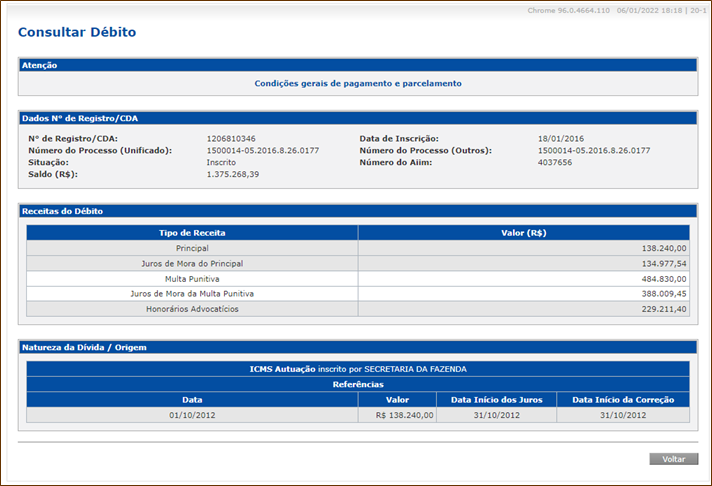
\includegraphics[width=1\textwidth]{Imagens/CDA n 1206810346 acostada a fl. 349 dos autos.png}
    \caption{CDA n° 1206810346 acostada à fl. 349 dos autos (emitida em 06/01/2021)}
    \label{fig:my_label}
\end{figure}


\begin{addmargin}[6cm]{} % Adiciona margim de recuo no texto

É possível observar que, a CDA supracitada foi emitida com posição de 06/08/2021, considerando que, nesta data, o valor de juros de mora da multa punitiva remonta em R\$ 388.009,45 sobre o valor principal da multa de R\$ 484.830,00, ou seja, depreende-se que o percentual de juros aplicado é de 80,04\%.
    \begin{itemize}
        \item \textbf{Qual foi a Taxa SELIC acumulada neste mesmo período?}

    \textbf{Resposta:} Considerando que se trata de novo posicionamento temporal de comparação, a \textbf{Perícia} perseguiu a Taxa SELIC acumulada considerando os parâmetros de termo inicial (outubro de 2012) e data do posicionamento da CDA de fl. 349 (agosto de 2021), na própria fonte de cálculo dos débitos tributários administrados pela União (sítio da Receita Federal do Brasil ), constatando que, a Taxa SELIC acumulada perfaz \textbf{74,79\%} para o mesmo período, vejamos:

\begin{figure}[!h]
    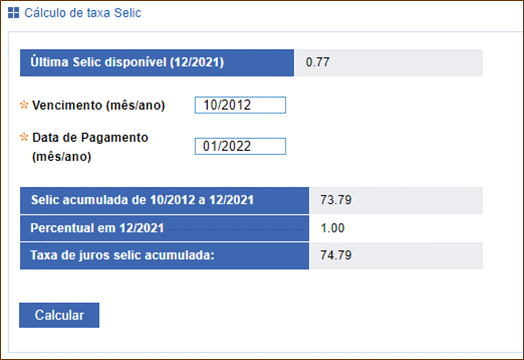
\includegraphics{Imagens/Taxa SELIC acumulada extraída do SICALC (Programa de Atualização Débitos da RFB).png}
    \caption{Taxa SELIC acumulada extraída do SICALC (Programa de Atualização Débitos da RFB)}
    \label{fig:my_label}
\end{figure}

%\newgeometry{left = 8cm} %muda a margem esquerda para 5cm
 \item \textbf{Podemos afirmar que os percentuais aplicados pela FESP para cálculo dos juros de mora da multa punitiva são superiores à Taxa SELIC?}
\textbf{Resposta:} Positiva é a resposta. Em virtude da aplicação da taxa de \textbf{80,04\%} em detrimento dos limites da Taxa SELIC acumulada, a qual resultou em \textbf{74,79\%} para o mesmo período.

\item \textbf{Podemos afirmar que ao aplicarmos a Taxa SELIC para cálculo dos juros de mora da multa punitiva o valor final efetivamente devido pela Autora a título de juros de mora da multa punitiva será reduzido?}

\textbf{Resposta:} Positiva é a resposta, aplicando a taxa de \textbf{74,79\%} identificada no próprio programa que acumula a Taxa SELIC e que remunera os débitos federais (tese da \textbf{Requerente}), o resultado dos juros de mora da multa punitiva perfaz o montante de \textbf{R\$ 350.252,70} já considerando que o percentual de \textbf{74,79\%} seja aplicado sobre a multa punitiva recalculada no valor de \textbf{R\$ 468.314,88}, sendo inferior ao montante calculado originalmente na CDA de fl. 349 dos autos, em referência ao quanto perquirido no quesito.
%\newgeometry{left = 3cm}
\end{itemize}
\end{addmargin}

